\documentclass[]{aa} %bibnumber

%\usepackage{hyperref}
\usepackage{txfonts}
\usepackage{amsmath}
\usepackage[colorlinks,breaklinks]{hyperref}
\hypersetup{linkcolor=blue,citecolor=blue,filecolor=black,urlcolor=blue}


\usepackage{color}
\newcommand{\mr}[1]{{\textcolor[rgb]{0.60,0.10,0.6}{#1}}}
\newcommand{\mri}[1]{{\textcolor{red}{#1}}}
\newcommand{\nn}[1]{{\textcolor[rgb]{1, 0.27, 0}{#1}}}

\def\l{\lambda}\def\L{\Lambda}

\newcommand{\prob}[2]{\mathcal{P}\left( #1 \mid #2\right)}

\begin{document}
\title{Redshift evolution of the SN stretch distribution}

%\subtitle{II. An example text with infinitesimal scientific value whose title
%and subtitle may also be split}

\author{N. Nicolas\inst{1}
    \and M. Rigault\inst{2}
    \and R. Graziani\inst{2}     
    \and M. Briday\inst{1}
    \and Y. Copin\inst{1}    
    \and Y. Kim\inst{1}
}

%\offprints{R. Plemmons, \email{plemmons@...}}

\institute{Université de Lyon, F-69622, Lyon, France; Université de Lyon
    1, Villeurbanne; CNRS/IN2P3, Institut de Physique des Deux Infinis, Lyon
    \and Université Clermont Auvergne, CNRS/IN2P3, Laboratoire de
    Physique de Clermont, F-63000 Clermont-Ferrand, France.
}

\date{Received 2 November 1992 / Accepted 7 January 1993}

\abstract{Type Ia supernovae (SNe Ia) allow for the construction of the Hubble
    diagram, giving us information about the Universe's expansion and its
    fundamental components, one of which is dark energy. But systematic
    uncertainties are now starting to be limiting in our ability to measure
those parameters. In particular, the physics of SNe Ia is still mostly unknown,
and is thought not to change in time/with the redshift.}
    {In an attempt to reduce those uncertainties, we try to find an empirical
    law describing SNe Ia's length of explosion (stretch) evolution with the
redshift.}
    {We started by getting a complete sample representing all of the stretch
        distribution that Nature can give us, before using LsSFR measurements,
        an age tracer which evolution with redshift is known, that has been
        shown to have a strong correlation with the stretch. We compare their
        AICc, an estimator of the relative quality of statistical models that
    includes the number of free parameters, to determine which ones describe
best the data.}
    {Models with an evolution of the stretch with the redshift have a better
    AICc than the ones without.}
    {We find that implementing these models allows us to fit the data better
    than models without stretch evolution.}

\keywords{Cosmology -- Type Ia Supernova -- Systematic uncertainties}
\maketitle

\section{Introduction}

%\begin{figure*}
%    \centering
%    \subfigure[Method]{\label{fig:zdet}%        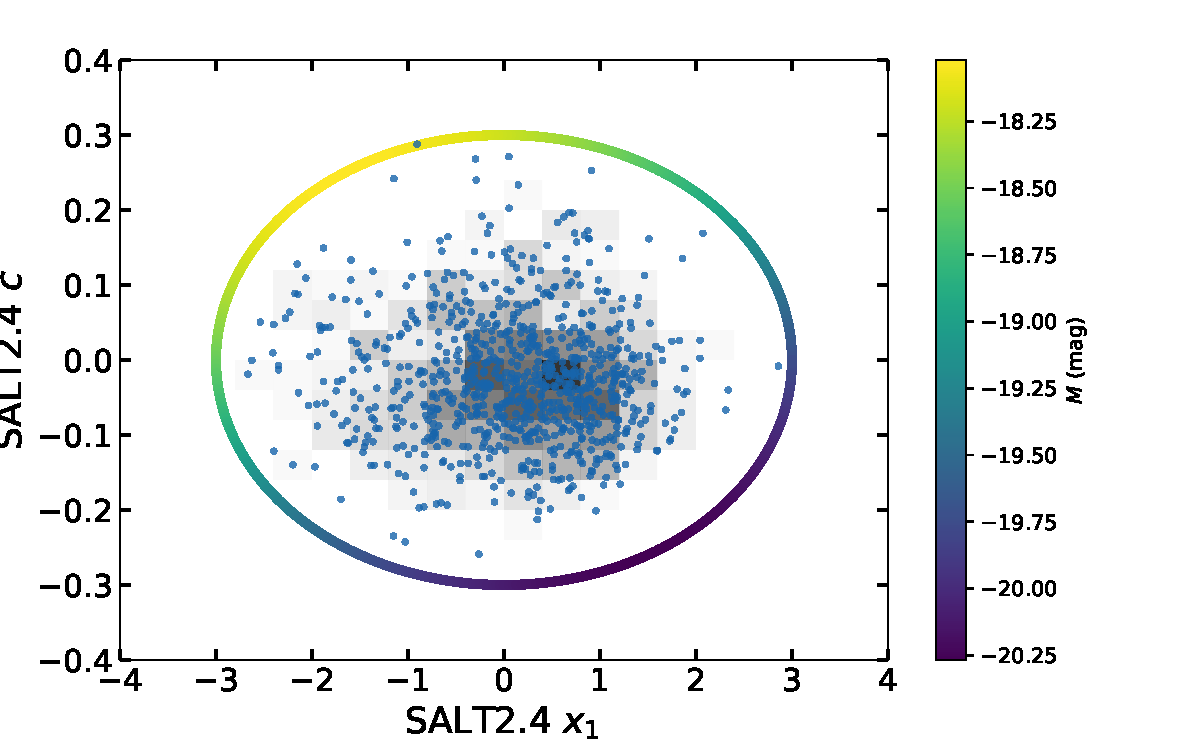
\includegraphics[width=8.5cm]{Article_figures/zmax_maglim_all.pdf}}


%        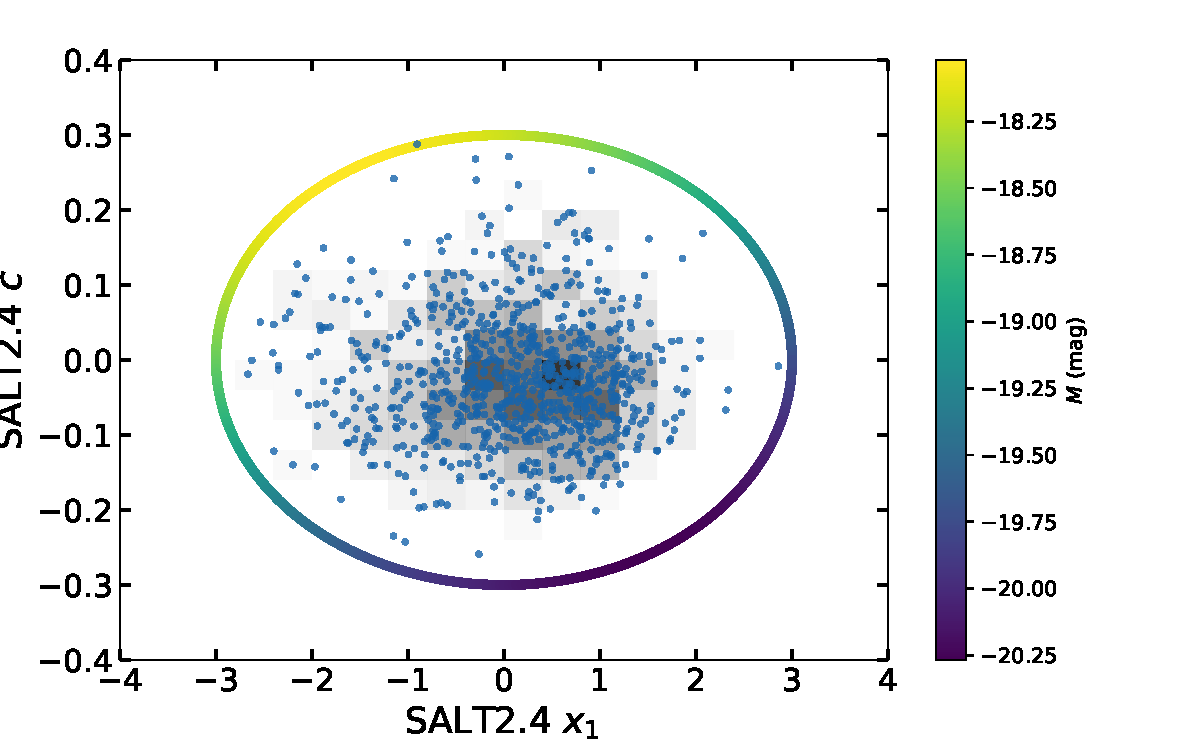
\includegraphics[width=8.5cm]{Article_figures/zmax_maglim_all.pdf}}
%    \subfigure[Result]{\label{fig:surveys_cuts}
%    \includegraphics[width=8.5cm]{A    \subfigure[Method]{\label{fig:zdet}
%rticle_figures/surveys_cuts_x.pdf}}
%    \subfigure[Method]{\label{fig:zdet}

%    \caption{(a) $z\St{max}$ determination from the magnitude limited data; (b) SDSS, %SNLS and PS1 samples cut at $z\St{max}$ as explained in
%    section \ref{sec:sam}. The data we use is in plain markers.}
%\subfigure[Method]{\label{fig:zdet}

%\end{figure*}

Type Ia supernovae (SNe Ia) are powerful cosmological distance indicators that
have enabled the discovery of the acceleration of the Universe's expansion
\citep{riess1998, perlmutter1999}. They remain today a key cosmological probe to
understand the properties of dark energy (DE) as it is the only tool able to
precisely map the recent expansion rate $z<0.5$, when DE is driving it
\citep[e.g.][]{scolnicastro2020}. They also are key to directly measure the
Hubble Constant (H$_0$) provided one can calibrate their absolute magnitude
\citep{riess2016, freedman2019}. Interestingly, the value of H$_0$ derived when
the SNeIa are anchored on Cepheids \citep[the SH0ES
project][]{riess2009,riess2016} is $\sim5~\sigma$ higher than what is predicted
by cosmic microwave background (CMB) data measured by Planck assuming the
standard $\L$CDM or when the SN luminosity is anchored at intermediate redshift
by the baryon acoustic oscillation (BAO) scale \citep{riess2019, reid2019,
planck2016, feeney} \nn{changed ried to reid; changed planck to planck2016;
feeney = https://tinyurl.com/vg6uufm ?}. While using the tip of the red giant
branch technique in place of the Cepheids seem to favor lower values of H$_0$
\citep{freedman2019, recalibrationpaper} \nn{changed "freedman" to
"freedman2019" ; recalibrationpaper = ?} time delay measurements from strong
lensing seem to also favor high H$_0$ values \citep{wong2019}.

The H$_0$ tension has received a lot of attention as it could be a sign of new
fundamental physics. Yet, no simple solution is able to accommodate this H$_0$
tension when accounting for all other probes and the current most promising
scenario appears to be a burst of expansion at the matter-radiation decoupling
moment caused by a (fine tuned) early dark energy \citep{poulin2019} \nn{changed
"poulin" to "poulin 2019"}.

Alternatively, systematic effects affecting one or several of the aforementioned
analysis could also explain the tension. In \cite{rigault2015} we suggested that
SNe Ia from the Cepheid calibrator sample differ significantly to the one from
the Hubble flow sample that enables to derive H$_0$. Indeed, Cepheid are very
young stars and the existence of Cepheids in a galaxy implies that the host is
star forming. In \citep{rigault2015} we claimed that a more than 90\% of the
calibrator SNe Ia arise from a young-progenitor population while this population
only accounts for about half of the Hubble flow sample. Following
\cite{sullivan2010} and \citep{rigault2013} \nn{should use cite or citep?}, we
further showed that young and old progenitor SNe Ia have a different magnitude
of about 0.15 mag. This has been confirmed for modern standardization technique
\citep[SALT2.4][]{guy2010,betoule2014} with high significance ($\sim 6\sigma$)
in \citep{rigault2018} as well as independently by \cite{roman2019} \nn{not
found on ADS: https://tinyurl.com/uemattg} at $\sim 7\sigma$. As detailed in
\citep{rigault2015}, if the magnitude difference between young and old SNe Ia is
indeed of $0.15$ mag and if SNe Ia from the calibrator sample is fully dominated
by young SNeIa, the effect on H$_0$ of the existence of these two SNe Ia
populations is of 3.5\%. Accounting for the fact that another environmental
effect (the mass-step) is already included in the SH0ES analysis, the net bias
in the SH0ES analysis is expected closer to 3\% \citep[see table 6
of][]{rigault2015}. 

SHOULD BE SHORTENED A LOT: However, the importance of this astrophysical bias in
the direct measurement of H$_0$ is still highly debated. We also highlight that
it could not explain the high value of H$_0$ derived by strong lensing. First,
\cite{jones2015} \nn{put the ref but nos sure it's the correct one} did not find
any environmental bias when extending the \citep{rigault2015} study. It was more
recently reported in \citep{jones2019} \nn{put the ref but nos sure it's the
correct one} that indeed local host analysis has significant influence on the SN
magnitude but much more importantly than claimed in \citep{rigault2018} and with
a connection with the progenitor physics and/or a line of sight effect that is
unclear. More importantly, \cite{riess2016} attended to mimic the Cepheid sample
selection function on the Hubble flow sample by removing SNe Ia from the latter
if they classified their host as early-type or non-star forming. They measured
that doing so has no effect on the measurement of H$_0$.

This paper is part of a series of papers where we test the validity of the two
SNe Ia population models developed in \citep{rigault2018}.Briday et al. in prep
will present how using different environmental tracer is affecting our ability
to distinguish the two populations, and Rigault et al. in prep will further
study the connection with H$_0$. Here we analyze predictions concerning the SNe
Ia redshift drifts: (1) that the distribution of the SNIa stretch, a purely
intrinsic SNIa property, is evolving as a function of redshift and (2) that this
population-drift follows the relation that \citep{rigault2018} derived assuming
that one population is “young“ with a rate proportional to the star formation
rate in the Universe and the second is "old" with a rate proportional to the
stellar mass.

The concept of the SNeIa age dichotomy arised when the SNIa rate has first been
studied. \cite{mannucci2005, scannapieco2005, sullivan2006, aubourg2008} have
shown that the relative SNe Ia rate in galaxies could only be explained if two
populations existed, one young, following the host star formation activity, and
one old following the host stellar mass (the so called “prompt and delayed“ or
“A+B“ model). In \cite{rigault2018} we used the specific star formation rate at
the SN location (Local sSFR or LsSFR) to classify which are the prompts (those
with a high LsSFR) and which are the delayed (those with low LsSFR). Since the
first SNe Ia host analysis, the SN stretch has been known to be strongly
correlated with the SN host properties \citep{hamuy1996, hamuy2000} \nn{put
hamuy1996 as most cited of https://tinyurl.com/sjlbdz8} and it has been
extensively confirmed since \citep[e.g.][]{neill2009, sullivan2010,
lampeitl2010, kelly2010, gupta2011, dandrea2011, childress2013, rigault2013,
pan2014} \nn{added all the refs}. Following the “A+B“ model and the connection
between SN stretch and host properties, \citep{howell2009} \nn{changed
howell20xx to howell2009
(https://ui.adsabs.harvard.edu/abs/2009ApJ...691..661H/abstract)} first
discussed the potential redshift drift of the SN stretch distribution. In this
paper we revisit this analysis with the most recent SNe Ia dataset and we test
the validity of the two SNIa age populations model developed by
\citep{rigault2018}.

We present in section~\ref{sec:sample} the sample we are using for this
analysis, which is based on the pantheon dataset \citep{scolnic2018a}. We
discuss the importance of obtaining a "complete" sample, i.e. representative of
the true underlying SNe Ia distribution, and how we build one from the Pantheon
sample.  We then present in section~\ref{sec:modeling} our modeling of the
distribution of stretch as a function of redshift based on the relative stretch
distribution of young and old SNeIa. Our results are presented in
section~\ref{sec:results} where we test if the distribution of stretch does
evolve as a function of redshift and if the age-model is in good agreement with
this evolution. We discuss our results and conclude in section~\ref{sec:ccl}.

Throughout the paper we use the Planck 2015 cosmology from the astropy library.

\section{A "complete" Sample}
\label{sec:sample}

We base our analysis on the latest SNe Ia compilation: the Pantheon catalog from
\cite{scolnic2018a}.  \mr{TO BE REPHRASED} Using this dataset, we aim at probing
if the average stretch, an intrinsic SN Ia property, evolves as a function of
redshift or not; the underlying question being that of the SNIa population
redshift drift.  The stretch has been shown to depend on the SN environment star
formation activity
\citep[e.g.][]{howell2007,sullivan2010,childress2013,rigault2013,rigault2018}
and because the star formation rate is about 40 times larger at the high
redshift end of the pantheon sample than at its lower redshifts
\citep[e.g.,][and references therein]{tasca2015}, one might think that simply
comparing the redshifts distribution in a few bins of redshift could be
sufficient to probe any SN stretch redshift drift.  In practice, selection
effects are affecting the observed SN stretch distributions, which could
significantly differ from the true underlying one if these selection effects
become significant. Indeed, because the observed SNIa magnitude correlates with
the lightcurve stretches (and colors) the first SNIa that such a survey will
miss will the reddest and the lowest-stretch ones. Consequently, if selection
effects is not accounted for, one might confuse true population drift with
selection effect and conversely.

In a magnitude limited survey, providing sufficient (and random) spectroscopic
follow-up for acquiring typing and host redshift, the selection effects should
be negligible bellow a given redshift where all SNe Ia, even the faintest, could
be observed.  In contrast, targeted surveys have highly complex selection
functions and we will discard them from our analysis. Fortunately, modern SN
cosmology sample such has the pantheon dataset are now dominated by magnitude
limited survey.

We present fig.~\ref{fig:maglim} the lightcurve stretch and color distributions
of SNeIa from these surveys, namely: PanStarrs \citep[PS1][]{ref}, the Sloan
Digital Sky Survey \citep[SDSS][]{ref} and the SuperNovae Legacy Survey
\citep[SNLS][]{astier2006}.  An ellipse in the salt2.4 $(x_1, c)$ plan with
major axis $x_1=3$ and manor axis $c=0.3$ encapsulates the full distribution
(see also \citealt{bazin2011} and \citealt{campbell2013} for a similar contour
but using a less conservative $c=0.2$ for the latter). Assuming the SN absolute
magnitude with $x_1=0$ and  $c=0$ is $M=-19.36$ \citep{kessler2009,scolnic2014}
we can derive the absolute standardized magnitude at maximum of light along the
aforementioned ellipse given the standardization coefficient $\alpha=0.16$ and
$\beta=3.14$ from \cite{scolnic2018a}.  The faintest SNIa is that with
$x_1=-1.66$ and $c=0.25$ and has an absolute standardized magnitude at peak in
Bessel-b band of $-18.31\,\mathrm{mag}$. Since we need to see this object
typically a week before and 10 days after peak to build a suitable lightcurve,
the effective absolute limiting magnitude therefore is
$\sim-18.00\,\mathrm{mag}$.  Hence, given the $5\sigma$ point source detection
magnitude limit of a magnitude limited survey, one can derive the maximum
redshift above which the faintest SNeIa will start to be missed.

\begin{figure}
    \centering
    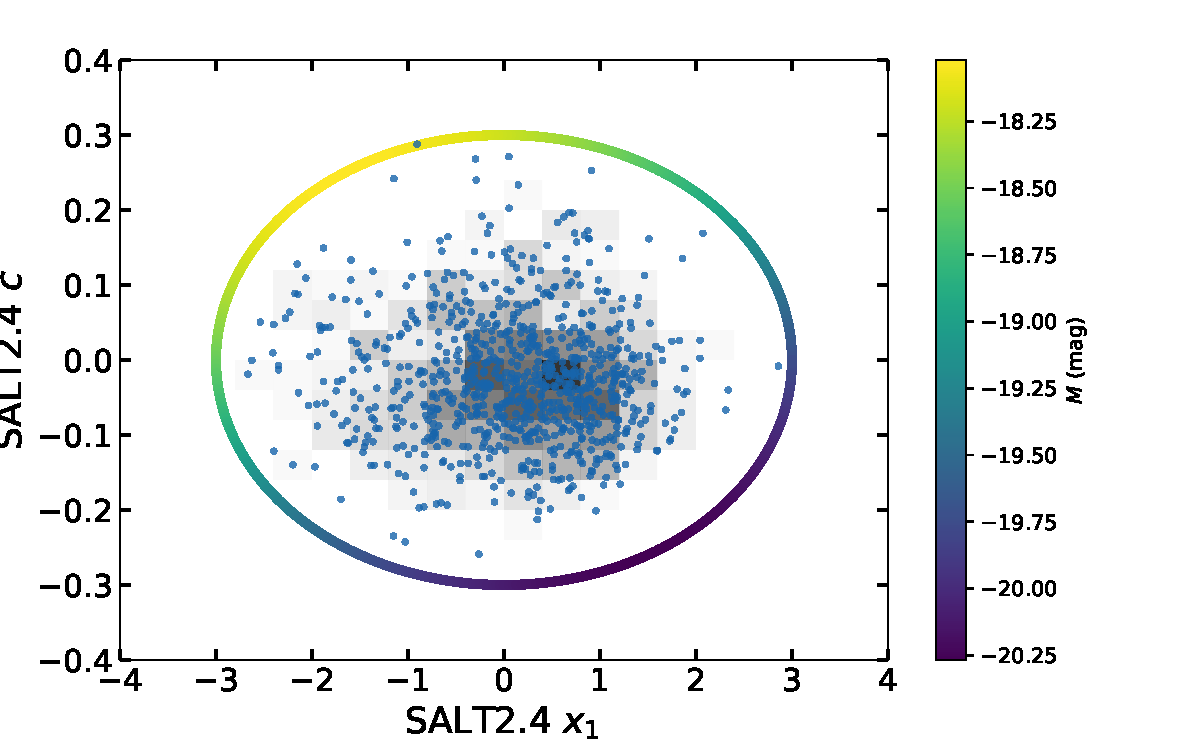
\includegraphics[width=\linewidth]{Article_figures/zmax_maglim_all.pdf}
    \caption{SALT2.4 stretch and color lightcurve parameters of SNeIa from the
        SDSS, PS1 and SNLS samples from the pantheon catalog. The individual SN
        data are shown as blue dots and a 2D histogram is shown in gray to
        highlight point density. The ellipse encapsulating all the SN data is
        displayed colored by the effective standardized absolute magnitude using
    the $\alpha$ and $\beta$ standardization coefficients from
\citep{scolnic2018a}.}
    \label{fig:maglim}
\end{figure}

SNLS typically acquires SNeIa in the redshift range $0.4<z<0.8$. At these
redshifts the rest-frame Bessel-b band roughly corresponds to the SNLS-$i$
filter that has a 24.8 mag $5\sigma$
depth\footnote{\href{https://www.cfht.hawaii.edu/Science/CFHTLS/cfhtlsfinalreleaseexecsummary.html}{CFHT
final release website.}}. This converts to a $z_{lim}=0.60$, in perfect
agreement with \cite{neill2006}, \cite{perrett2010} and \cite{bazin2011}.
Similarly, PS1 observes SNeIa in the range $0.2<z<0.4$, their $g$-band $5\sigma$
depth is 23.1 mag \citep{rest2014}, which yields to $z_{lim}=0.30$.  Figure~6 of
\citep{scolnic2018a} suggests a more conservative $z_{lim}$ of 0.27 for the PS1
catalog.  In similar redshift range, SDSS has a limiting magnitude of 22.5
\citep{dilday2008,sako2008}, which would lead to a $z_{lim}=0.24$. However, the
SDSS survey were more sensitive to limited spectroscopic resources.
\cite{kessler2009} present that during year-1 of SDSS, SNeIa with $r-mag<20.5$
were favored for spectroscopic follow up, corresponding to the redshift cut at
$0.15$. For the rest of the SDSS survey, additional spectroscopic resources were
used, such that \cite{kessler2009} and \cite{dilday2008} show a relative
completeness up to $z_{lim}=0.2$.  Following these analysis we will use
$z_{lim}=0.2$ as the baseline SDSS redshift limit for the rest of the analysis.
We could have chosen more conservative redshift limits for each of these
surveys, namely $z_{lim}=0.15$ for SDSS, $z_{lim}=0.27$ for PS and
$z_{lim}=0.55$ for SNLS, following Fig.~14 of \citealt{perrett2010}, and we will
also present results obtained when doing so.  We present the redshift
distribution of these three surveys in fig.~\ref{fig:cuts}, where we see that
the redshift limit roughly correspond to the pick of these histograms, as
expected.

\begin{figure}
    \centering
    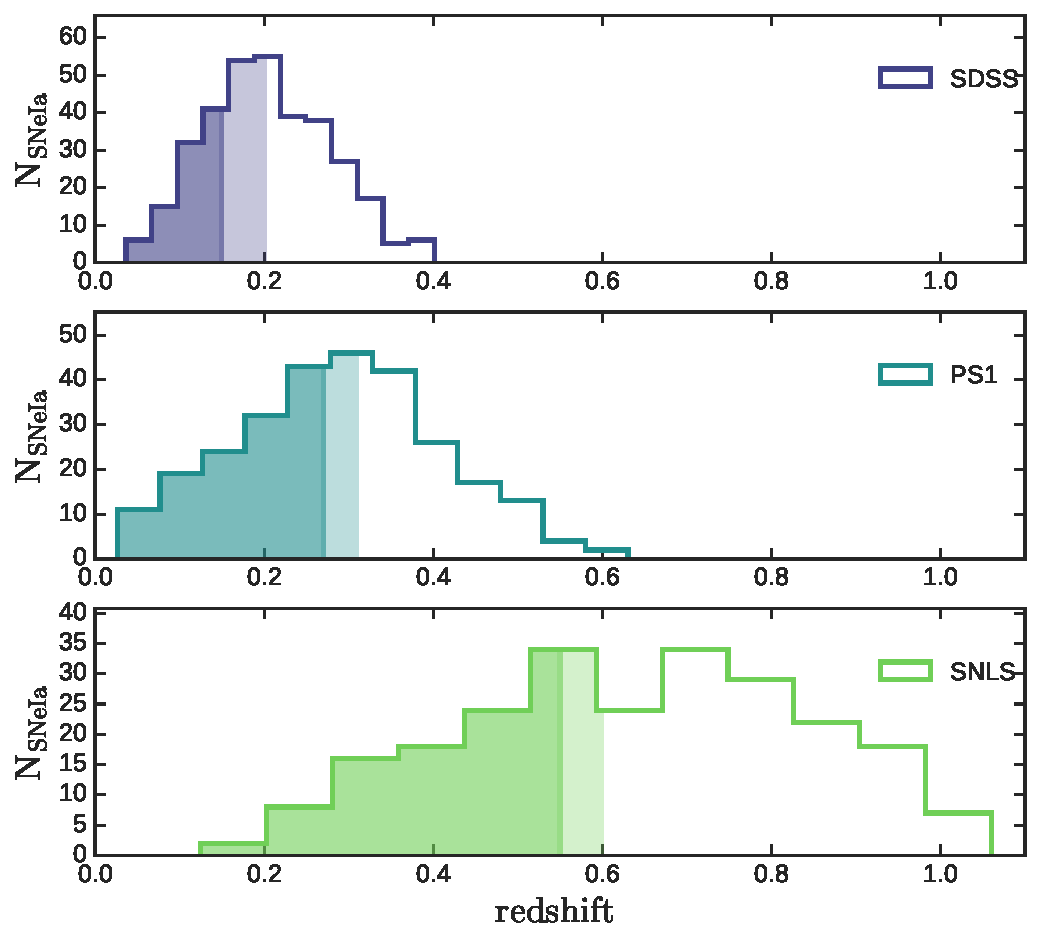
\includegraphics[width=\linewidth]{Article_figures/hist_surveys_cuts.pdf}
    \caption{Histograms of the 3 surveys on which we applied cuts to get rid of
    selection effects, as discussed in section \ref{sec:sample}. The SNe Ia
between the conservative and non-conservative cuts are shown in transparent.}
    \label{fig:cuts}
\end{figure}

In addition, we use the SNeIa from the nearby supernovae factory
\citep[SNfactory][]{aldering2004} \nn{added ref assuming
https://ui.adsabs.harvard.edu/abs/2004APS..APR.V4003A/abstract} published in
\citep{rigault2018} and that have been discoverd from no-targeted survey (114
SNeIa, see their section~3 and 4.2.2). As the SNe search were much deeper than
the spectrophotometric follow-up, SNfactory SNe Ia within a redshift range of
$0.02<z<0.09$ should also be a random sampling of the underlying SN population.
Data from \citep{rigault2018} are within these redshift boundaries. The HST
sample from Pantheon follows the same logic and we therefore kept it entirely
\citep{FIND BACK THE REF} \nn{lots of choices: https://tinyurl.com/rcsx7cw}.

\begin{table}
    \centering
    \caption{Source surveys of SNeIa used in our "complete" sample. Conservative
    cuts are indicated in brackets.}
    \label{tab:sample}
    \begin{tabular}{l c c}
    \hline\hline\\[-0.8em]
        Survey & N$_{\mathrm{SN}}$  & z$_{max}$ \\[0.15em]
        \hline\\[-0.8em]
        SNf & 114 & --\\[0.30em]
        SDSS & 167(82) & 0.20(0.15)\\[0.30em]
        PS1 & 160(122) & 0.30(0.27) \\[0.30em]        
        SNLS & 102(78) & 0.60(0.55)\\[0.30em]
        HST & 26 & --\\[0.30em]
        \hline
    \end{tabular}
\end{table}


%%%%%%%%%%%%%%%%%%%%%%%
%   LITERATURE        %
%%%%%%%%%%%%%%%%%%%%%%%
%\mri{COMPARE HERE WITH LITERATURE. E.G. FIG. 6 OF SCOLNIC 2018, PS zmax
%AROUND0.27}

%\mri{Perrett et al. 2010 | SNLS | zmax ="z $\sim$ 0.6"}

%\mri{Dilday et al. 2008 | SDSS | sure good at z<0.12, fig. 10 suggest still
%okat z=0.2}

%\mri{Kessler 2009 "For the SDSS-II, the image-subtraction
%pipeline efficiency (	subtr) is complete up to a redshift of z ∼ 0.2"}

%\mri{Kesslet 2009 | "For the SDSS-II and SNLS samples, the cutoff redshifts are
%estimated to be 0.15 and 0.65, respectively."}
% ADDIND: PS cut from pantheon close to 0.27 see Fig. 6 of Scolnic 2018

%%%%%%%%%%%%%%%%%%%%%%%
%       INFO          %
%%%%%%%%%%%%%%%%%%%%%%%
%Fraction of random SDSS stretchs being < mean_conservative =  0.299
%Fraction of random PS1 stretchs being < mean_conservative =  0.254
%Fraction of random SNLS stretchs being < mean_conservative =  0.417



\section{Modeling the redshift drift}
\label{sec:modeling}

In \cite{rigault2018} we presented a modeling of the evolution of the fraction
of prompt and delayed SNeIa as a function of redshift following former work on
rates and delay time distributions; see e.g. the prompt and delayed SNeIa model,
aka the "A+B" model,
\cite{mannucci2005,scannapieco2005,sullivan2006,aubourg2008} and
\cite{maozmannucci2014} for a review on delay time distributions of SNeIa. In
short, we assume that the number of prompt SNeIa follows the star formation
activity in the Universe while the number of delayed SNeIa follows the number of
Gyr-old stars in the Universe, i.e. the stellar mass. Hence, if we denote
calling $\delta(z)$ (resp. $\phi(z)$) the fraction of young (resp. old) SNeIa in
the Universe as a function of redshift, then their ratio is expected to follow
the evolution of the specific star formation rate which goes as $(1+z)^{2.8}$
until $z\sim2$ \citep{tasca2015}. Hence since there is  $\sim50\%$ of young
SNeIa at $z\sim0.05$ \citep{rigault2013,rigault2018}, in agreement with rate
expectations \citep{mannucci2006,rodney2014}, then, we find in
\cite{rigault2018}:
\begin{align}
    \label{eq:delta}
    \delta(z) & = \left( K^{-1} \times (1+z)^{-2.8} +1 \right)^{-1}\,
                  \mathrm{or,}\\
    \psi(z) & = \left( K \times (1+z)^{+2.8} +1 \right)^{-1},
\end{align}

where $K=0.87$ given the fraction of young in the SNfactory sample. This
modelisation is comparable to the evolution predicted by \cite{childress2014}
based on SN rates in galaxies depending on their quenching time as a function of
their stellar mass.

\subsection{With LsSFR data}
\label{sec:modelpy}

In \cite{rigault2018} we present that the SN stretch is strongly correlated with
the LsSFR, which traces age. We present this correlation in
fig.~\ref{fig:stretchlssfr}. To model the evolution of the SN stretch as a
function of redshift given our aforementioned model of the evolution of the
fraction of young (old) SNeIa, we need to model the SN stretch distribution of
each age sample. Given the structure of the stretch--LsSFR scatter plot show
fig.~\ref{fig:stretchlssfr}, we define our model as follows: for the young
population the underlying stretch distribution is modeled as $\mathcal{N}(\mu_1,
\sigma_1)$, i.e. a normal distribution centered on $\mu_1$ with a $\sigma_1$
width ; the old population stretch distribution is  modeled as $a\times
\mathcal{N}(\mu_1, \sigma_1) + (1-a)\times \mathcal{N}(\mu_2, \sigma_2)$, i.e. a
gaussian mixture where one mode is the same as the young population one.  The
estimation of the 5 free parameters
($\theta\equiv{\mu_1,\mu_2,\sigma_1,\sigma_2,a}$) of the model is given by
minimizing:
\begin{equation}
    \label{eq:likelihood}
    \mathcal{L} = -2 \sum_i \ln\left( \prob{x^{i}_{1}}{\theta\ ;
                     \mathrm{d}x^{i}_{1}, p(y)^{i}}\right),
\end{equation}
with
\begin{align}
    \label{eq:likelihoodsnf}
    \prob{x^{i}_{1}}{ \theta\ ; \mathrm{d}x^{i}_{1}, p(y)^{i}} = 
    p(y)^{i}\,\times\,&\mathcal{N}\left(\mu_1, \sqrt{\sigma_1{}^{2}
    +\mathrm{d}x^{i}_{1}{}^{2}}\right)(x^{i}_{1})\,+\nonumber\\
    (1-p(y)^{i}) \times [a\,\times\,& \mathcal{N}\left(\mu_1,
    \sqrt{\sigma_1{}^{2}+\mathrm{d}x^{i}_{1}{}^{2}}\right)(x^{i}_{1})\,
    + \nonumber\\
    (1-a)\,\times\,&\mathcal{N}\left(\mu_2, \sqrt{\sigma_2{}^{2}
    +\mathrm{d}x^{i}_{1}{}^{2}}\right)(x^{i}_{1})\,],
\end{align}
where $i$ is the index of the SNIa, $x^{i}_{1}$, $\mathrm{d}x^{i}_{1}$ and
$p(y)^{i}$ are the salt2.4 stretch, error of the salt2.4 stretch and the
probability that the SN is prompt, respectively.  In practice, since "$a$" is
defined between 0 and 1, we fit for $\alpha$ such that
$a=\arctan(\alpha)/\pi+0.5$, which results into asymmetric error on $a$.

\begin{figure*}
    \label{fig:stretchlssfr}
    \centering
      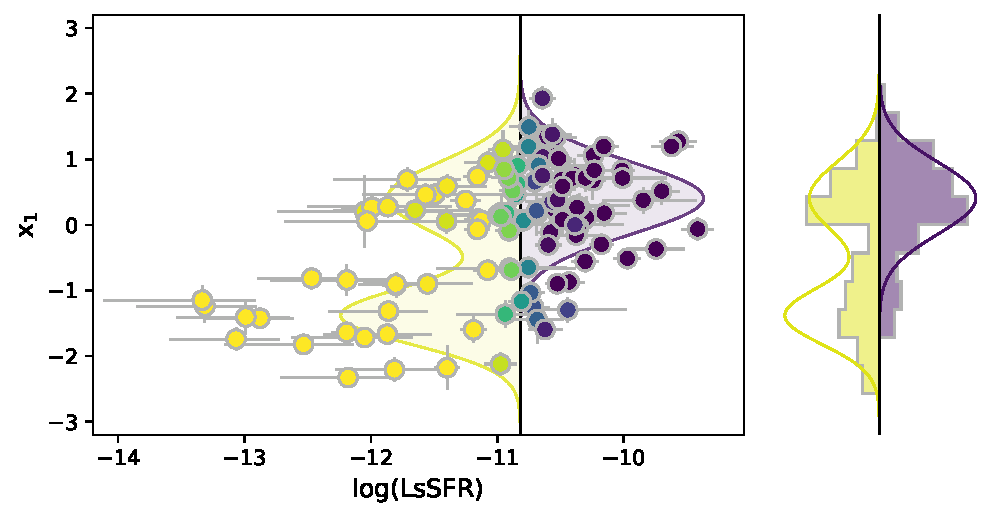
\includegraphics[width=\linewidth]{Article_figures/BiGaussian_hist.pdf}
    \caption{SNF data on which we based our models of stretch distribution
    between young and old}
\end{figure*}

The fit results are shown table~\ref{tab:modelresults} and the best fit model is
illustrated in fig.~\ref{fig:stretchlssfr}.

\begin{table*}
    \centering
    \caption{Best fit value of the stretch distribution model. The "SNf" results
    are derived using eq.~\ref{eq:likelihoodsnf} solely using the SNf data for
which we have $p(y)$. The "All" and "All(cons)" results are derived using
eq.~\ref{eq:likelihood} without the age information (see
section~\ref{sec:modelnopy}) ; "All(cons)" correspond to the "complete sample"
using conservative redshift cut (see section~\ref{sec:sample}).}
    \label{tab:modelresults}
    \begin{tabular}{l c c c c c}
    \hline\hline\\[-0.8em]
        Sample & $\mu_1$  & $\sigma_1$ &$\mu_2$  & $\sigma_2$ & a \\[0.15em]
        \hline\\[-0.8em]
        SNf & $0.41 \pm 0.08$ & $0.55 \pm 0.06$ & $-1.38 \pm 0.10$ &
        $0.44 \pm 0.08$ & $0.48^{+0.08}_{-0.08}$ \\[0.15em]
        All & $0.43 \pm 0.09$ & $0.58 \pm 0.05$ & $-1.05 \pm 0.28$ &
        $0.63 \pm 0.13$ & $0.51^{+0.09}_{-0.10}$ \\[0.15em]
        All(cons) & $0.38 \pm 0.05$ & $0.60 \pm 0.06$ & $-1.26 \pm 0.13$
                  & $0.53 \pm 0.08$ & $0.47^{+0.09}_{-0.08}$ \\[0.15em]
        \hline
    \end{tabular}
\end{table*}

When combining our prediction of the evolution of young SNeIa as a function of
redshift eq.~\ref{eq:delta}, and the stretch distribution of the both the young
and the old SNeIa, our model for the underlying distribution of stretch
$\Delta\left(x_1|z\right)$ as a function of redshift is:
\begin{align}
    \label{eq:stretchz}
    \Delta\left(x_1\,|\,z \right) = 
    &\,\delta(z)\times\mathcal{N}(\mu_1,\sigma_1)\,+\nonumber\\
    (1-&\,\delta(z)) \times \left[a\times\mathcal{N}(\mu_1,\sigma_1)
    + (1-a)\times\mathcal{N}(\mu_2,\sigma_2)\right]
\end{align}

\subsection{Without LsSFR data}
\label{sec:modelnopy}

Given eq.~\ref{eq:stretchz}, we can extend the analysis by fitting the free
parameters of the model ($\theta\equiv{\mu_1,\mu_2,\sigma_1,\sigma_2,a}$)
assuming the evolution of the fraction of young SNeIa as a function of redshift
given by $\delta(z)$ and given, this time, $x_1^{i}$,  $\mathrm{d}x^{i}_{1}$ and
$z^{i}$, the stretch, error on the stretch and redshift of any given SN $i$. In
practice, it means that we are still minimizing for the same
eq.~\ref{eq:likelihood}, but replacing $p(y)^{i}$ by $\delta(z^{i})$
eq.~\ref{eq:likelihoodsnf}. 

The fit results when using the conservative redshift cuts or not are shown
table~\ref{tab:modelresults} and the best fit models are illustrated in
fig.~\ref{fig:modelall}.
 
\begin{figure*}
    \centering
    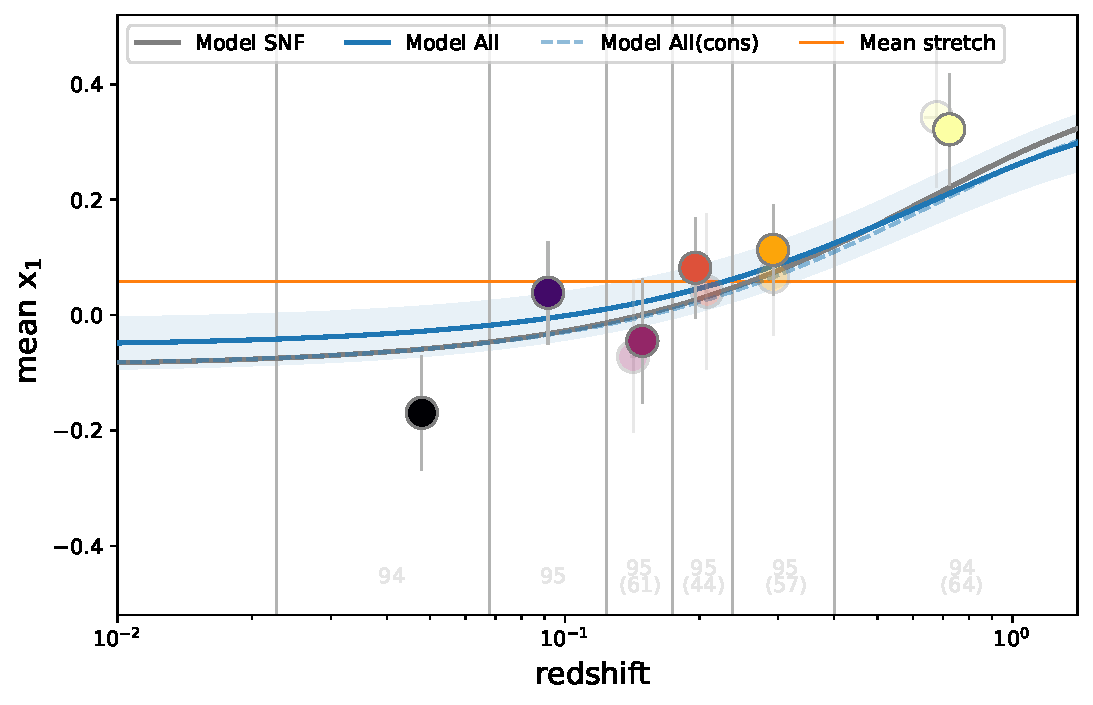
\includegraphics[width=\linewidth]{Article_figures/stretchevol_all_vs_snf_maglim-cuts.pdf}
    \caption{Result of the model fitted on all the surveys' data, cut at the
    conservative $z_{\mathrm{max}}$ in transparent and non-conservative
$z_{\mathrm{max}}$ in full markers. The number of SNe Ia in each bin is
indicated just above the x-axis in transparent text; between brackets are the
numbers for the conservative cuts.}
    \label{fig:modelall}
\end{figure*}

\subsection{Other modelings}
\label{sec:othermodel}

In section~\ref{sec:modelpy} and \ref{sec:modelnopy} we have modeled the
underlying stretch distribution as a single gaussian for the young SNe Ia and a
combination of two gaussians for the old SNe Ia population, i.e., the same as
the young-population one plus another for the fast declining SNeIa that seem to
only exist in old populations.

\cite{howell2007} used a simpler modelisation: the underlying stretch of each
age population is a single gaussian. This rises the question of the accuracy of
our modeling choice. To test this, we have implemented a suite of extra
parametrisation that we also fit to the data following the procedure described
section~\ref{sec:modelnopy}. Namely we consider:
\begin{itemize}

    \item "Base$+(\mu_1^{\mathrm{O}}, \sigma_1^{\mathrm{O}})$": base model but
        where the high-stretch Gaussian of the old population is not set as that
        of the young population ;

    \item "Base$-(\sigma_2)$": base model but where $\sigma_2$ is fixed at the
        same value as $\sigma_1$, since both width seem not significantly
        different in Table~\ref{tab:modelresults};

    \item "Howell": one single Gaussian per age group as in \citep{howell2007},
        but with the $\delta(z)$ factor.

\end{itemize}

Furthermore, since we aim at probing the SN redshift drift, we are also fitting
the "Base" model and the three aforementioned extensions by fixing the
population drift parameter $\delta(z)$ to a free parameter constant
$\delta(z)=f$. Doing so enables us to consider two last models. The first is
modeling the underlying SNe Ia stretch distribution by a simple Gaussian, namely
"Gaussian (f)". The second is using an asymmetric Gaussian distribution as
currently done by the BBC formalism introduced by \cite{kessler2017,
scolnic2018b} for modeling the sample selection functions in SN Cosmology. This
last model is particularly interesting to test as it is currently used in the
most recent SN Cosmological analyses \cite{riess2016, riess2018, PSpaper,
scolnic2018a, DESpaper} \nn{supposed riess2018 to be
https://ui.adsabs.harvard.edu/abs/2018ApJ...861..126R/abstract}; see further
discussion concerning this issue in section~\ref{sec:bbc}.

The ability of the model to explain the data is detailed in
section~\ref{sec:results}.

\section{Results}
\label{sec:results}

We applied each model on both the conservative and non-conservative sample (cf.
section \ref{sec:sample}. We want to test whether including an evolution of the
stretch with the redshift ($\delta(z)$ factor) would better describe the data.
As the various models presented section~\ref{sec:modeling}, have various degrees
of freedom. To compare them all, we use the Akaike Information Criterion
corrected for sample size (AICc), that penalizes extra degrees of freedom to
avoid over-fitting the data. The AICc is defined as follow:
\begin{equation}
    \mathrm{AICc} = \mathrm{AIC} + \frac{2k\left(k+1\right)}{n - k - 1}
\end{equation}

with $\mathrm{AIC} = 2k + \mathcal{L}$, where $k$ is the number of free
parameters and $\mathcal{L}$ is defined eq~\eqref{eq:likelihood}.  The best
model is the one with the smaller AICc and the probability for another model to
be at least as representative of the data as this one is given by:
\begin{equation}
    p(\mathrm{other} > \mathrm{best}) = \exp\left(\Delta\mathrm{AICc}/2\right)
\end{equation}
The results are summarized in table \ref{tab:comp} and represented figure
\ref{fig:mod_comp}.

\begin{table*}
    \centering
    \caption{Comparison of quality of fit for all the models. Base indicates the
    models designed for this study. (F) indicates models without an evolution of
the fraction of young SNe Ia as a function of the redshift.}
    \label{tab:comp}
    \begin{tabular}{c c c  c c c c  c c c c}\hline\hline\\[-0.8em]
        & & & \multicolumn{4}{c}{All SNeIa (569)} &
        \multicolumn{4}{c}{All SNeIa (conservative ; 422)} \\
        %\cline{2-6}
        Name & drift(?) & Free param &
        $\ln\mathcal{L}$ & $\mathrm{AICc}$ & $\Delta \mathrm{AICc}$ & Proba &
        $\ln\mathcal{L}$ & $\mathrm{AICc}$ & $\Delta \mathrm{AICc}$ & Proba \\
        [0.15em]\hline\\[-0.8em]

        Base$-(\sigma_2)$ & $\delta(z)$ & 4
        & 1456.9 & 1464.9 & -- &  --
        & 1079.9 & 1088.0 & -- & -- \\[0.15em]

        Base & $\delta(z)$ & 5
        & 1456.7  & 1466.8 & -1.8 & $4.0\times10^{-1}$
        & 1079.5 & 1089.6 & -1.7 & $4.4\times10^{-1}$\\[0.15em]

        Base$+(\mu_1^{\mathrm{O}}, \sigma_1^{\mathrm{O}})$ & $\delta(z)$ & 7
        & 1453.1  & 1467.3 & -2.4 & $3.1\times10^{-1}$
        & 1074.5 & 1088.8 & -0.8 & $6.7\times10^{-1}$\\[0.15em]

        Howell & $\delta(z)$ & 4
        & 1463.3 & 1471.3 & -6.4 & $4.1\times10^{-2}$
        & 1088.2 & 1096.3 & -8.3 & $1.5\times10^{-2}$\\[0.15em]

        Assymetric & $f$ & 3
        & 1485.2 & 1491.3 & -26.3 & $1.9\times10^{-6}$
        & 1101.3 & 1107.4 & -19.4 & $6.2\times10^{-5}$\\[0.15em]

        Howell & $f$ & 5
        & 1484.2 & 1494.3 & -29.4 & $4.2\times10^{-7}$
        & 1101.2 & 1111.3 & -23.4 & $8.5\times10^{-6}$\\[0.15em]
        
        Base$+(\mu_1^{\mathrm{O}}, \sigma_1^{\mathrm{O}})$ & $f$ & 8
        & 1478.9 & 1495.2 & -30.2 & $2.8\times10^{-7}$
        & 1095.5 & 1111.9 & -23.9 & $6.5\times10^{-6}$\\[0.15em]

        Base & $f$ & 6
        & 1484.2 & 1496.4 & -31.4 & $1.5\times10^{-7}$
        & 1101.2 & 1113.4 & -25.4 & $3.0\times10^{-6}$\\[0.15em]

        Gaussian & -- & 2
        & 1521.8 & 1525.8 & -60.9 & $6.0\times10^{-14}$
        & 1142.6 & 1146.6 & -58.6 & $1.9\times10^{-13}$ \\[0.15em]

        Base$-(\sigma_2)$ & $f$ & 5
        & 1521.8 & 1531.9 & -67.0 & $2.9\times10^{-15}$
        & 1142.6 & 1152.7 & -64.7 & $8.8\times10^{-15}$\\\hline

    \end{tabular}
\end{table*}

\begin{figure*}
    \centering
    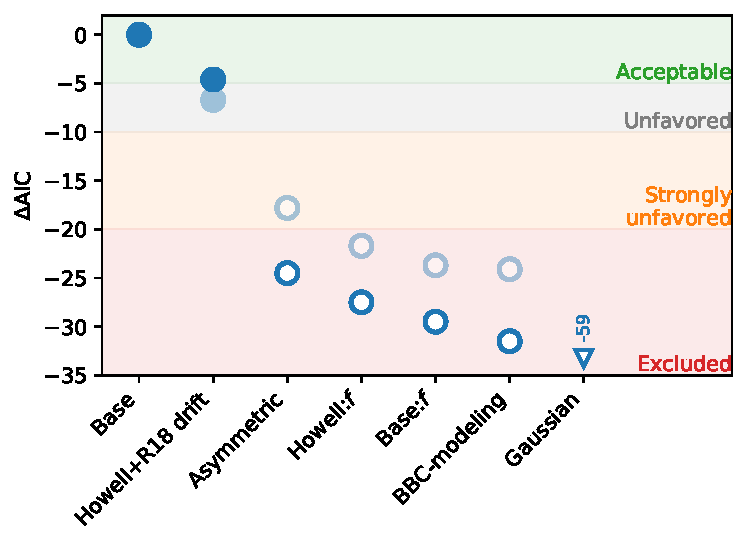
\includegraphics[width=\linewidth]{Article_figures/mod_comp.pdf}
    \caption{$\Delta$AICc of the models fitted on all the surveys' data, cut at
    the conservative $z_{\mathrm{max}}$ in transparent and non-conservative
$z_{\mathrm{max}}$ in full markers.}
    \label{fig:mod_comp}
\end{figure*}

For the non-conservative part, we find that every model lacking an evolution of
the stretch with the redshift is systematically worse than those that implement
it, and that removing the $\sigma_2$ parameter gives better results than letting
it free, or adding $(\mu_1^{\mathrm{O}}, \sigma_1^{\mathrm{O}})$. However, the
base model with 2 gaussians for the old population is roughly the same as the
Howell model with one gaussian per population. As for the conservative part, all
the models but the asymmetric and the gaussian ones correctly fit the data. No
fixed model fit better than those with evolution, but some come close. It would
seem that taking SNe Ia close to us doesn't give us a sample where the evolution
is visible, justifying the study done in section~\ref{sec:sample}.

\section{discussion}

\subsection{BBC and assumptions on underlying SN property}
\label{sec:bbc}
BBC use the asymmetric model. When we do it, we get the table TABLE

\begin{table*}
    \centering
    \caption{Fit results of the asymmetric and base models for the 3 surveys
    having selection effects.}
    \label{tab:bbc}
    \begin{tabular}{c c c c c c c c c c}\hline\hline\\[-0.8em]
    Asymetric & Free param & $\sigma^-$ & $\sigma^-_{\mathrm{err}}$ &
    $\sigma^+$ & $\sigma^+_{\mathrm{err}}$ & $\mu^0$ & $\mu^0_{\mathrm{err}}$
               & ln $\mathcal{L}$ & AICc \\\hline
    SDSS & 3 & 1.25 & 0.08 & 0.39 & 0.07 & 0.69 & 0.10 & 893.9 & 900.0 \\
    PS1 & 3 & 1.00 & 0.09 & 0.49 & 0.09 & 0.42 & 0.12 & 702.0 & 708.1 \\
    SNLS & 3 & 1.18 & 0.11 & 0.39 & 0.11 & 0.81 & 0.15 & 594.8 & 600.9 \\\hline
    Total & 9 & -- & -- & -- & -- & -- & -- & 2190.7 & 2209.0\\\hline
    \end{tabular}
    
    \vspace*{12pt}
    
    \begin{tabular}{c c c c c}\hline\hline\\[-0.8em]
    Base &  Free param & ln $\mathcal{L}$ & AICc \\\hline
    SDSS & 0 & 395.2 & 405.6 \\
    PS1 & 0 & 444.7 & 455.0 \\
    SNLS & 0 & 254.1 & 264.7 \\\hline
    Total & 0 & 1094.0 & 1125.4 \\\hline
    \end{tabular}
\end{table*}

\section{Conclusion}
\label{sec:ccl}
Stretch evolution with the redshift is a thing. Need to see if it has an impact
on the cosmology though.

\begin{acknowledgements}
This project has received funding from the European Research Council (ERC) under
the European Union's Horizon 2020 research and innovation programme (grant
agreement n 759194 - USNAC). 

    % How has received that support for this project ? 
    %Support has been provided by the Institut Universitaire de France, the CNES, and the region Auvergne-Rhone-Alpes.
\end{acknowledgements}

\bibliographystyle{aa} % style aa.bst
\begin{thebibliography}{} 
% A
\bibitem[Abbott et al.(2018)]{abbott2018} Abbott, T.~M.~C., Abdalla, F.~B., Alarcon, A., et al.\ 2018, \prd, 98, 043526

\bibitem[Aldering(2004)]{aldering2004} Aldering, G.\ 2004, APS April Meeting Abstracts 2004, V4.003

\bibitem[Astier et al.(2006)]{astier2006} Astier, P., Guy, J., Regnault, N., et al.\ 2006, \aap, 447, 31


\bibitem[Ata et al.(2017)]{ata2017} Ata, M., Kitaura, F.-S., Chuang, C.-H., et al.\ 2017, \mnras, 467, 3993

\bibitem[Aubourg et al.(2008)]{aubourg2008} Aubourg, {\'E}.,
  Tojeiro, R., Jimenez, R., et al.\ 2008, \aap, 492, 631 


% B
\bibitem[Betoule et al.(2014)]{betoule2014} Betoule, M., Kessler, R., Guy, J., et al.\ 2014, \aap, 568, A22

\bibitem[Bazin et al.(2011)]{bazin2011} Bazin, G., Ruhlmann-Kleider, V., Palanque-Delabrouille, N., et al.\ 2011, \aap, 534, A43

% C
\bibitem[Campbell et al.(2013)]{campbell2013} Campbell, H., D'Andrea, C.~B., Nichol, R.~C., et al.\ 2013, \apj, 763, 88


\bibitem[Chabanier et al.(2019)]{chabanier2019} Chabanier, S., Millea, M., \& Palanque-Delabrouille, N.\ 2019, \mnras, 489, 2247

\bibitem[Childress et al.(2013)]{childress2013} Childress, M., Aldering, G., Antilogus, P., et al.\ 2013, \apj, 770, 108

\bibitem[Childress et al.(2014)]{childress2014} Childress, M.~J., Wolf, C., \& Zahid, H.~J.\ 2014, \mnras, 445, 1898


\bibitem[Coles, \& Jones(1991)]{coles1991} Coles, P., \& Jones, B.\ 1991, \mnras, 248, 1


% D
\bibitem[D'Andrea et al.(2011)]{dandrea2011} D'Andrea, C.~B., Gupta, R.~R., Sako, M., et al.\ 2011, \apj, 743, 172

\bibitem[Dilday et al.(2008)]{dilday2008} Dilday, B., Kessler, R., Frieman, J.~A., et al.\ 2008, \apj, 682, 262


% E
% F
\bibitem[Freedman et al.(2019)]{freedman2019} Freedman, W.~L., Madore, B.~F., Hatt, D., et al.\ 2019, \apj, 882, 34

% G
\bibitem[Gupta et al.(2011)]{gupta2011} Gupta, R.~R., D'Andrea, C.~B., Sako, M., et al.\ 2011, \apj, 740, 92

\bibitem[Guy et al.(2010)]{guy2010} Guy, J., Sullivan, M., Conley, A., et al.\ 2010, \aap, 523, A7

%\bibitem[Graziani et al.(2019)]{graziani2019} Graziani, R., Courtois, H.~M., Lavaux, G., et al.\ 2019, \mnras, 488, 5438

% H
\bibitem[Hamuy et al.(1996)]{hamuy1996} Hamuy, M., Phillips, M.~M., Suntzeff, N.~B., et al.\ 1996, \aj, 112, 2391

\bibitem[Hamuy et al.(2000)]{hamuy2000} Hamuy, M., Trager, S.~C., Pinto, P.~A., et al.\ 2000, \aj, 120, 1479

\bibitem[Howell et al.(2007)]{howell2007} Howell, D.~A., Sullivan, M., Conley, A., et al.\ 2007, \apjl, 667, L37

\bibitem[Howell et al.(2009)]{howell2009} Howell, D.~A., Sullivan, M., Brown, E.~F., et al.\ 2009, \apj, 691, 661

% I 
% J
\bibitem[Jones et al.(2015)]{jones2015} Jones, D.~O., Riess, A.~G., \& Scolnic, D.~M.\ 2015, \apj, 812, 31

\bibitem[Jones et al.(2018)]{jones2018} Jones, D.~O., Riess, A.~G., Scolnic, D.~M., et al.\ 2018, \apj, 867, 108

\bibitem[Jones et al.(2019)]{jones2019} Jones, D.~O., Scolnic, D.~M., Foley, R.~J., et al.\ 2019, \apj, 881, 19

% K
\bibitem[Kelly et al.(2010)]{kelly2010} Kelly, P.~L., Hicken, M., Burke, D.~L., et al.\ 2010, \apj, 715, 743

\bibitem[Kessler et al.(2009)]{kessler2009} Kessler, R., Becker, A.~C., Cinabro, D., et al.\ 2009, \apjs, 185, 32

\bibitem[Kessler, \& Scolnic(2017)]{kessler2017} Kessler, R., \& Scolnic, D.\ 2017, \apj, 836, 56

\bibitem[Knox, \& Millea(2019)]{knox2019} Knox, L., \& Millea, M.\ 2019, arXiv e-prints, arXiv:1908.03663

% L
\bibitem[Lampeitl et al.(2010)]{lampeitl2010} Lampeitl, H., Smith, M., Nichol, R.~C., et al.\ 2010, \apj, 722, 566

% M
\bibitem[Mannucci et al.(2005)]{mannucci2005} Mannucci, F.,
  Della Valle, M., Panagia, N., et al.\ 2005, \aap, 433, 807 
\bibitem[Mannucci et al.(2006)]{mannucci2006} Mannucci, F.,
  Della Valle, M., \& Panagia, N.\ 2006, \mnras, 370, 773 

\bibitem[Maoz et al.(2014)]{maozmannucci2014} Maoz, D., Mannucci,
  F., \& Nelemans, G.\ 2014, \araa, 52, 107 


% N
\bibitem[Neill et al.(2006)]{neill2006} Neill, J.~D., Sullivan, M., Balam, D., et al.\ 2006, \aj, 132, 1126

\bibitem[Neill et al.(2009)]{neill2009} Neill, J.~D., Sullivan, M., Howell, D.~A., et al.\ 2009, \apj, 707, 1449

% O
% P
\bibitem[Pan et al.(2014)]{pan2014} Pan, Y.-C., Sullivan, M., Maguire, K., et al.\ 2014, \mnras, 438, 1391

\bibitem[Perlmutter et al.(1999)]{perlmutter1999} Perlmutter, S., Aldering, G., Goldhaber, G., et al.\ 1999, \apj, 517, 565

\bibitem[Perrett et al.(2010)]{perrett2010} Perrett, K., Balam, D., Sullivan, M., et al.\ 2010, \aj, 140, 518

\bibitem[Planck Collaboration et al.(2016)]{planck2016} Planck Collaboration, Ade, P.~A.~R., Aghanim, N., et al.\ 2016, \aap, 594, A13

\bibitem[Poulin et al.(2019)]{poulin2019} Poulin, V., Smith, T.~L., Karwal, T., et al.\ 2019, \prl, 122, 221301

\bibitem[Planck Collaboration et al.(2018)]{planck2018} Planck Collaboration, Aghanim, N., Akrami, Y., et al.\ 2018, arXiv e-prints, arXiv:1807.06209

% Q
% R
\bibitem[Reid et al.(2019)]{reid2019} Reid, M.~J., Pesce, D.~W., \& Riess, A.~G.\ 2019, arXiv e-prints, arXiv:1908.05625

\bibitem[Rest et al.(2014)]{rest2014} Rest, A., Scolnic, D., Foley, R.~J., et al.\ 2014, \apj, 795, 44

\bibitem[Riess et al.(1998)]{riess1998} Riess, A.~G., Filippenko, A.~V., Challis, P., et al.\ 1998, \aj, 116, 1009

\bibitem[Riess et al.(2009)]{riess2009} Riess, A.~G., Macri, L., Casertano, S., et al.\ 2009, \apj, 699, 539

\bibitem[Riess et al.(2016)]{riess2016} Riess, A.~G., Macri, L.~M., Hoffmann, S.~L., et al.\ 2016, \apj, 826, 56

\bibitem[Riess et al.(2018)]{riess2018} Riess, A.~G., Casertano, S., Yuan, W., et al.\ 2018, \apj, 861, 126

\bibitem[Riess et al.(2019)]{riess2019} Riess, A.~G., Casertano, S., Yuan, W., et al.\ 2019, \apj, 876, 85

\bibitem[{Rigault {et~al.}(2013)}]{rigault2013}
Rigault, M., Copin, Y., Aldering, G., {et~al.} 2013, \aap, 560, A66

\bibitem[Rigault et al.(2015)]{rigault2015} Rigault, M., Aldering, G., Kowalski, M., et al.\ 2015, \apj, 802, 20


\bibitem[Rigault et al.(2018)]{rigault2018} Rigault, M.,
  Brinnel, V., Aldering, G., et al.\ 2018, arXiv:1806.03849

\bibitem[Rodney et al.(2014)]{rodney2014} Rodney, S.~A.,
  Riess, A.~G., Strolger, L.-G., et al.\ 2014, \aj, 148, 13 


% S
\bibitem[Sako et al.(2008)]{sako2008} Sako, M., Bassett, B., Becker, A., et al.\ 2008, \aj, 135, 348

\bibitem[Scannapieco \& Bildsten(2005)]{scannapieco2005} Scannapieco, E., \& Bildsten, L.\ 2005, \apjl, 629, L85 

\bibitem[Scolnic et al.(2014)]{scolnic2014} Scolnic, D., Rest, A., Riess, A., et al.\ 2014, \apj, 795, 45

\bibitem[Scolnic et al.(2018)]{scolnic2018a} Scolnic, D.~M., Jones, D.~O., Rest, A., et al.\ 2018a, \apj, 859, 101

\bibitem[Scolnic et al.(2018)]{scolnic2018b} Scolnic, D.~M., Lochner, M., Gris, P., et al.\ 2018, arXiv e-prints, arXiv:1812.00516

\bibitem[Scolnic et al.(2019)]{scolnicastro2020} Scolnic, D., Perlmutter, S., Aldering, G., et al.\ 2019, Astro2020: Decadal Survey on Astronomy and Astrophysics, 2020, 270

\bibitem[Sullivan et al.(2006)]{sullivan2006} Sullivan, M., Le  Borgne, D., Pritchet, C.~J., et al.\ 2006, \apj, 648, 868 


\bibitem[Sullivan et al.(2010)]{sullivan2010} Sullivan, M., Conley, A., Howell, D.~A., et al.\ 2010, \mnras, 406, 782

% T
\bibitem[Tasca et al.(2015)]{tasca2015} Tasca, L.~A.~M., Le F{\`e}vre, O., Hathi, N.~P., et al.\ 2015, \aap, 581, A54

% U 
% V
% W
\bibitem[Wong et al.(2019)]{wong2019} Wong, K.~C., Suyu, S.~H., Chen, G.~C.-F., et al.\ 2019, arXiv e-prints, arXiv:1907.04869

% X
% Y
 Z
\end{thebibliography}


\end{document}





%%%%%%%%%%%%%%%%%%%%%%%%
%
%  BACKUP 
%
%%%%%%%%%%%%%%%%%%%%%%%%


%For clarity with the next models, we named it 3G2M2S$_{\text{SNf}}$ for it has a total of 3 gaussians but with only 2 means and 2 standard deviations, and has been fitted on SNf data only. 

%We implemented and compared 10 models in total, 4 of which have an
%evolution with the redshift from $\delta(z)$, and 6 don't ($\delta(z) = f =\mathrm{cst}$). The ones with and evolution are:
\begin{itemize}
    \item 3G2M2S, the one we described (but fitted on all the data);
    \item 3G2M1S, where this time $\sigma_1 \equiv \sigma_2$;
    \item 2G2M2S, model taken from HOWELL 2009 where we added $\delta(z)$;
    \item 3G3M3S, with three independent gaussians.
\end{itemize}
The ones without a stretch evolution are the same ones but with an "F" implying
we set $\delta(z) = f = \mathrm{cst}$, and two others:
\begin{itemize}
    \item 1G1M1S, where there is no distinction between old and young SNe;
    \item 1G1M2S, taken from KESLLER 2017 and used in recent cosmological
        analysis SCOLNIC 2018. It's an asymetric model where
\end{itemize}
\begin{align}
 p(x_1^i, \mathrm{d} x_1^i | \mu, \sigma_-, \sigma_+) = 
    \begin{cases}
        \mathcal{N} \left(\mu, \sqrt{\sigma_-{}^2 + \mathrm{d} x_1^i{}^{2}}\right) (x_1^i) & \text{if
        } x_1^i\geq \mu\\
        \mathcal{N} \left(\mu, \sqrt{\sigma_+{}^2 + \mathrm{d} x_1^i{}^{2}}\right) (x_1^i), &
        \text{else}
    \end{cases}
\end{align} 

The fitted parameters are showed table \ref{tab:val}.

\begin{table*}[htbp!]
    \centering
    \caption{Values of the best-it parameters for all the models. In red are the non-coherent ones which coincides with the models without an evolution of the fraction of young SNe Ia with the redshift.}
    \label{tab:val}
    \begin{tabular}{c c c c c c c}\hline\hline

        Model & $a$ & $f$ & $\mu_1$ & $\sigma_1$ & $\mu_2$ &
        $\sigma_2$ \\\hline

        3G2M2S$_{\mathrm{SNf}}$ & $0.48 \pm 0.07$ & none & $0.39 \pm 0.07$ &
        $0.56 \pm 0.05$ & $-1.5 \pm 0.1$ & $0.52 \pm 0.09$ \\

        3G2M2S & $0.48 \pm 0.17$ & none & $0.36 \pm 0.08$ & $0.61 \pm 0.05$ &
        $-1.3 \pm 0.2$ & $0.60 \pm 0.12$ \\

        3G2M2SF & \textcolor{red}{$0.1 \pm 0.6$} & \textcolor{red}{$0.2 \pm
        0.6$} & $-0.9 \pm 0.7$ & $0.7 \pm 0.3$ & $0.5 \pm 0.2$ & $0.6 \pm 0.1$
        \\

        3G2M1S & $0.47 \pm 0.07$ & none & $0.35 \pm 0.04$ & $0.61 \pm 0.03$ &
        $-1.25 \pm 0.10$ & $\sigma_1$ \\

        3G2M1SF & \textcolor{red}{$0.2 \pm 0.9$} & $0.7 \pm 0.3$ & $0.36 \pm
        0.04$ & $0.60 \pm 0.03$ & $-1.23 \pm 0.10$ & $\sigma_1$ \\

        2G2M2S & none & none & $0.49 \pm 0.04$ & $0.54 \pm 0.03$ & $-0.72 \pm
        0.08$ & $0.83 \pm 0.07$ \\
        
        2G2M2SF & none & $0.3 \pm 0.2$ & $-0.9 \pm 0.6$ & $0.7 \pm 0.2$ & $0.5
        \pm 0.2$ & $0.56 \pm 0.09$ \\\hline

    \end{tabular} \bigbreak

\begin{tabular}{c c c}\hline\hline

    Model & $\mu$ & $\sigma$ \\\hline

    1G1M1S & $0.01 \pm 0.04$ & $0.90 \pm 0.03$ \\\hline

\end{tabular} \bigbreak

\begin{tabular}{c c c c c}\hline\hline

    Model & $\mu$ & $\sigma_-$ & $\sigma_+$ \\\hline

    1G1M2S & $0.16617 \pm 0.00004$ & $1.07 \pm 0.04$ & $0.69 \pm 0.03$ \\\hline

\end{tabular} \bigbreak

\begin{tabular}{c c c c c c c c c}\hline\hline

    Model & $a$ & $f$ & $\mu_1$ & $\sigma_1$ & $\mu_2$ & $\sigma_2$ &
    $\mu_3$ & $\sigma_3$ \\\hline

    3G3M3S & $0.14 \pm 0.08$ & none & $0.51 \pm 0.06$ & $0.54 \pm 0.04$ & $-1.9
    \pm 0.2$ & $0.29 \pm 0.11$ & $-0.55 \pm 0.12$ & $0.67 \pm 0.15$ \\
    
    3G3M3SF & $0.2 \pm 0.2 $ & $0.10 \pm 0.04 $ & $-1.7 \pm 0.2$ & $0.4 \pm 0.1$
            & $0.9 \pm 0.1$ & $0.3 \pm 0.2$ & $0.0 \pm 0.2$ & $0.7 \pm 0.1$
            \\\hline

\end{tabular} \bigbreak
\end{table*}

To test the coherence of this model, we also fitted it using all the data from the surveys indistinctly. These results are shown figure \ref{fig:model_all}.


